\documentclass[openany,overnay,a4paper, twoside, 12pt]{book}
\usepackage[document]{ragged2e} %para poder justificar el texto
\usepackage{float}
\usepackage{graphicx}
\usepackage[utf8]{inputenc}

\usepackage[noindentafter]{titlesec}
\usepackage{wrapfig}
\renewcommand\bibname{Bibliografía}
\usepackage{pdfpages}
\usepackage[document]{ragged2e} %para poder justificar el texto
\usepackage[a4paper,width=150mm,top=25mm,bottom=25mm,bindingoffset=10mm]{geometry} %igualar los margenes de las paginas pares e impares
\usepackage{hyperref} % ESTO HACE QUE EL INDICE TENGA ENLACES A LOS CAPITULOS
\renewcommand{\contentsname}{Índice} %Cambio el nombre de Content a Índice
\title{Cosa}
\author{María y Hector}
\date{February 2022}
\usepackage[utf8]{inputenc}
\usepackage[noindentafter]{titlesec}
\usepackage{wrapfig}
\usepackage{pdfpages}
\usepackage[document]{ragged2e} %para poder justificar el texto
\usepackage[a4paper,width=150mm,top=25mm,bottom=25mm,bindingoffset=10mm]{geometry} 
\title{\textbf{Soluciones ERP y CRM} \\
\\\\\
\newline
\newline
\newline
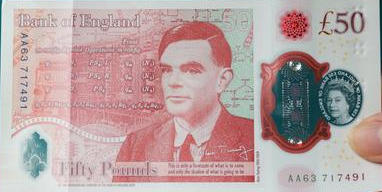
\includegraphics[scale = 0.8]{imagenes/att.png}}
%Añado la imagen justo antes en el titulo
\setlength{\parindent}{6.5ex} 




\author{
    Carcasona, Héctor\\
    Co-founder\\
    IES Ítaca\\
    6658hcarcasona@e-itaca.es
  \and
    Herrero, María\\
   Co-founder\\
    IES Ítaca\\
    0224mherrero@e-itaca.es}
\date{Febraury 2022}

\pagestyle{plain} %Para que los numeros de página aparezcan siempre en medio 
\begin{document}
\let\cleardoublepage\clearpage %Para evitar que se cree una página vacia (Valdrá solo con uno de esos comandos???)
\maketitle
\tableofcontents
\setcounter{chapter}{1}
\addcontentsline{toc}{chapter}{ERPs}
\chapter*{\centering ERPs}
\section{ERP Libre: Odoo, el ERP \textit{Todo en uno}}
\subsection{Información general}
Cuando hablamos de ERP libre, lo primero que nos viene a la cabeza es Odoo. \\Este se trata de ERP que engloba todo lo necesario para la empresa. Tiene dos versiones distintas, una cominutaria y otra empresarial, licenciadas bajo GNU LGPL v3, Odoo Enterprise Edition License v1.0, respectivamente.
\\
\subsection{Módulos y aplicaciones}
Enumerar todos los modulos y funcionalidades de este ERP es tarea imposible: Cuenta con decenas de módulos y más de 20.000 aplicaciones. Aunque, hay algunas características de estos que vale la pena destacar. 
\begin{itemize}
    \item Cubren una gran espectro de necesidades 
    \item Están en constante actualización 
    \item La cantidad y características de sus módulos convierten a Odoo en un ERP transversal. 
\end{itemize}
\\
 A continuación, hemos añadido una lista de algunos de sus módulos:
\begin{itemize}
    \item Accounting: Ddedicado a la contabilidad y facturación de la empresa
    \item Manufacturing: Dedicado a la manufacturación, controles de calidad, mantenimiento...
    \item eCommerce: Dedicado al sitio web, el comercio electrónico y la integración con páginas como Ebay. 
    \item Inventory: Dedicado al inventario y las compras necesarias. 
    \item Marketing: Dedicado a todo el tema de marketing, desde su planificación hasta su automatización.
    \item Sales: Dedicado al tema de ventas. Aquí se incluye el CRM de Odoo, además de subscripciones y registros.
    \item Shipping: Dedicado a los envíos. Incluye la integración con distintas empresas de paquetería
    \item Human Resources: Dedicado a recursos humanos: Bajas, contrataciones, jornadas...
\end{itemize}
\newpage

Un buen ejemplo sería: En la lista 'Odoo Shipping', se pueden encontrar módulos personalizados para las grandes empresas de paquetería (FedEx, DHL...).\\
Además, tiene módulos específicos para el internet de las cosas (IoT). Esta cantidad de módulos y aplicaciones permite que Odoo sea una solución para todo tipo de empresas, desde pequeñas hasta multinacionales.\\\\
\subsection{Hardware}
En el aspecto de hardware, destaca la posibilidad de utilizar una "IoT box", la cual sigue la misma lógica que el propio ERP: Servir como un todo en uno para los demás hardwares (Zebra, TPV...).\\
\subsection{Software}
En el plano de software, Odoo está orientado a objetos y está escrito en Python y JavaScript, mientras que su parte dedicada a las bases de datos funciona mediante PostgreSQL. \\
Utiliza un sistema servidor-cliente para balancear la carga de los procesos. Además, permite crear reportes unificados mediante herramientas como Jasper Reports. Por último, la información en Odoo está mostrada de forma dinámica mediante XML.\\
Odoo no tiene un máximo de usuarios concurrentes \textit{per se}, esto depende de la capacidad del servidor utilizado. Para ejemplificar, se han documentado hasta 50.000 usuarios simultáneos. \\\\
\subsection{Interfaz gráfica}
La interfaz gráfica de Odoo es muy sencilla y visual. \\La pantalla principal consiste en una distribución iconizada de los distintos módulos habilitados, lo cual permite tener un orden de la aplicación desde la primera vista.\\
Las interfaces dentro de los distintos módulos son similares: Una visión de la aplicación elegida en el plano general y, arriba, una selección de las aplicaciones principales del módulo.\\ A continuación, dos imágenes para ejemplificar: 
\begin{figure}[b]
    \centering
    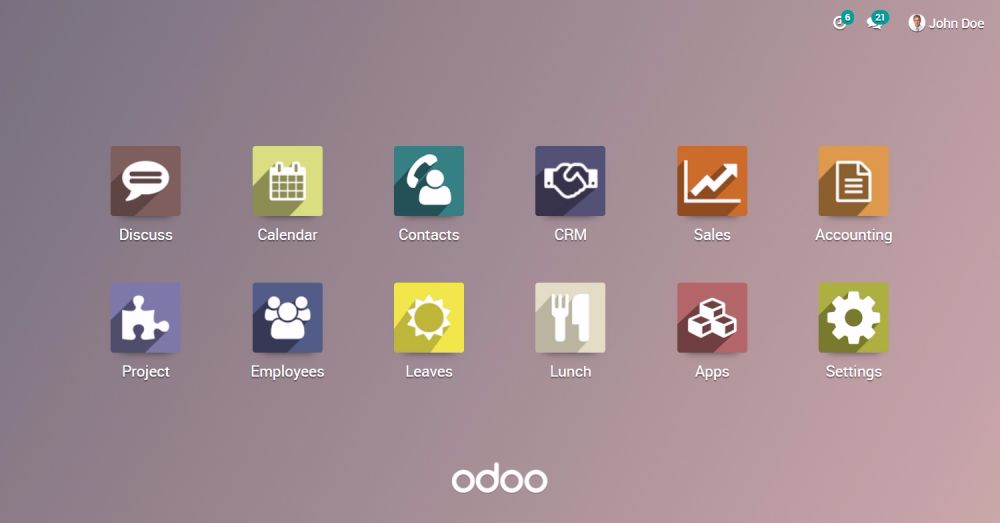
\includegraphics[scale=0.3]{sgeI/interfazPrincipal.jpg}
    \caption{Interfaz principal de Oboo}
    \label{fig:my_label}
\end{figure}
\begin{figure}[H]
    \centering
    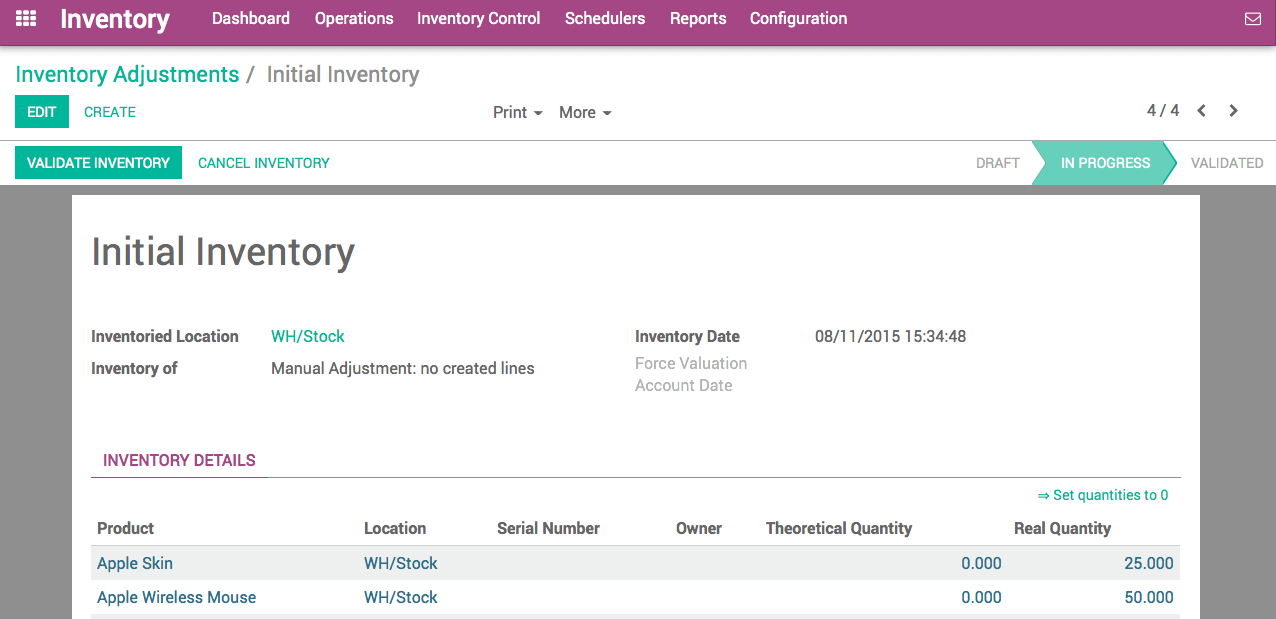
\includegraphics[scale=0.3]{sgeI/interfazInventario.jpg}
    \caption{Interfaz de inventario de Odoo}
    \label{fig:my_label}
\end{figure}
\newpage
\section{ERP Propietario: SAP ERP}
\subsection{Información general}
Este ERP, propiedad de la compañia SAP, es posiblemente uno de los más 'estrictos' en termino de propiedad. Su versión actual es la 6.0, la cual se mantiene con paquetes de mejoras, siendo el último el "EHP8 para SAP ERP 6.0". SAP tiene diferentes licencias para los diferentes usos que se les puede dar. Para utilizar este ERP necesitas una licencia de SAP y una conexión al servidor. \\
SAP es un entorno demandante, lo cual permite que varias empresas desconectadas entre si trabajen juntas. 
\subsection{Módulos y aplicaciones}
SAP tiene 25 módulos. Algunos de los más importantes son: 
\begin{itemize}
    \item Contabilidad financiera
    \item Gestión de la cadena de suministros
    \item Ventas
    \item Logística
    \item Recursos humanos
    \item Control de costes
    \item Planificación del producto
\end{itemize}
\subsection{Hardware} 
Para mantener el ERP se necesitan, aproximadamente, 85 GB de disco duro, dividiéndose de la siguiente forma: 
\begin{itemize}
    \item SAP ERP: 75 GB
    \item Instanciación primaria del servidor: 2 GB
    \item Instanciaciones adicionales del servidor: 2 GB
    \item ABAP central services instance (ASCS): 2 GB
\end{itemize}
Además, necesitarás aproximadamente 11 GB de RAM. 

En cuanto a las aplicaciones, SAP funciona mediante transacciones, en otras palabras, cada aplicación es creada como una transacción del usuario final, que recupera datos de los usuarios y realiza la acción requerida.
\newpage
\subsection{Software}
SAP está escrito en C, C++ y ABAP. Una de las cualidades de SAP es este último lenguaje, creado \textit{ex profeso} para este ERP. ABAP es una especie de lenguaje 'atrapalotodo' en el que se basa todo el ecosistema de SAP. \\Este lenguaje está orientado a objetos y es interpretado. \\ Su mayor particularidad es la transversalidad del lenguaje: Tiene características de lenguajes tan dispares como Java o COBOL, además de combinarse con sentencias OPEN SQL, lo cual le permite comunicarse con prácticamente cualquier base de datos. Este lenguaje tiene dos tipos de datos, completos e incompletos (Dependiendo de si debes darles el tamaño que tendrán). Para ejemplificar esto, aquí se pueden ver una lista de algunos datos completos
\begin{table}[h]
\begin{center}
\begin{tabular}{| r | l | c | c|}
\hline
Letra & Tipo & Tamaño & Ejemplo \\ \hline
D & Fecha & 8 & 2020/10/30 \\
T & Hora & 6 & 18:40:59 \\\hline
I & Integer & 4 bytes & 20 \\ 
F & float & 8 bytes & 2.40 \\\hline
\end{tabular}
\caption{Datos completos en ABAP}
La existencia de un tipo de dato para "Fecha" ejemplifica perfectamente las peculiaridades de este lenguaje y su conexión con las bases de datos. 

\end{center}
\end{table}
\subsection{Interfaz gráfica}
La interfaz de SAP está basada en tres niveles: 
\begin{itemize}
    \item Nivel de presentación (GUI)
    \item Nivel de aplicación 
    \item Nivel de base de datos
\end{itemize}
Estando la GUI en la parte del cliente y los demás en el servidor.\\
La conexión se realiza a traves de 'SAP Logon', donde, tras iniciar sesión con tus credenciales, llegarás a una pantalla así:
\newpage
\begin{figure}
    \centering
    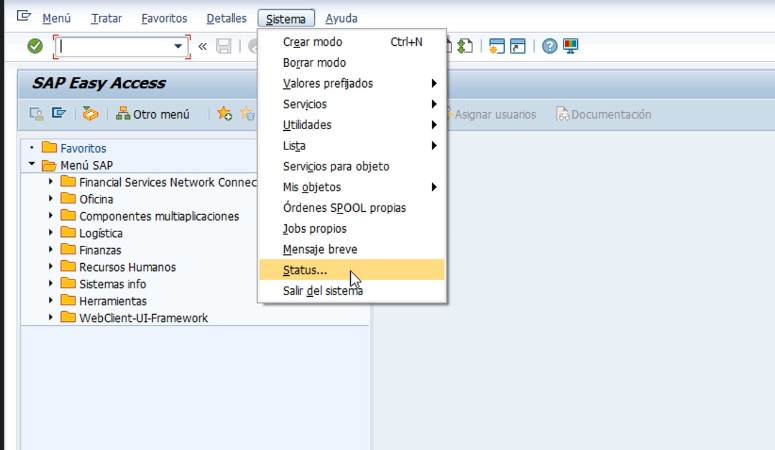
\includegraphics[scale=0.40]{sgeI/SAP.jpg}
    \caption{Interfaz principal de SAP}
    \label{fig:my_label}
\end{figure}
\begin{figure}[b]
    \centering
    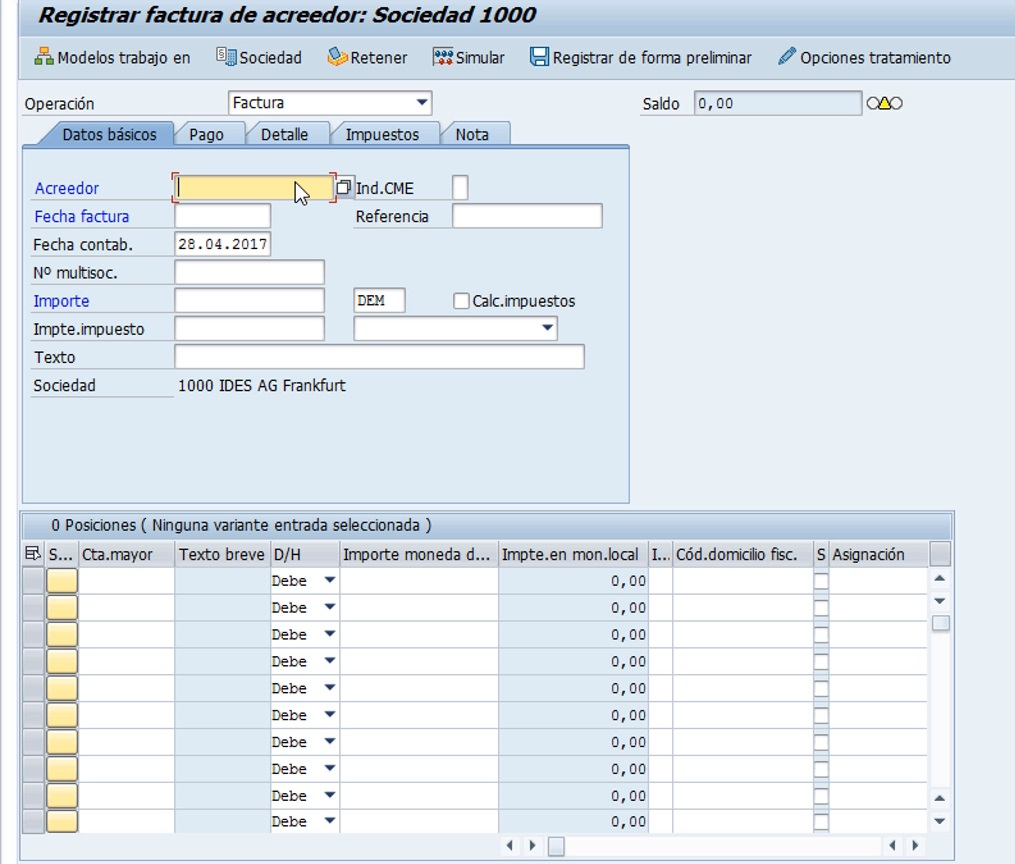
\includegraphics[scale=0.25]{sgeI/FacturaSAP.jpg}
    \caption{Interfaz durante la creación de una factura SAP}
    \label{fig:my_label}
\end{figure}
\addcontentsline{toc}{chapter}{CRMs}
\setcounter{chapter}{2}
\chapter*{\centering CRMs}
\setcounter{section}{0}
\section{CRM libre: SuiteCRM}
\subsection{Información general}
SuiteCRM surge debido a una bifurcación de SugarCRM, ya que este último pasó a ser software propietario. Está licenciado bajo \textit{GNU Lesser General Public License} y se encuentra en su versión 7.9.9. El programa es, en pocas palabras, la última versión libre de SugarCRM con varios módulos añadidos. Todas estas características hacen que la migración de SuiteCRM a SugarCRM sea sencilla, si así fuese necesario. 

\subsection{Módulos y aplicaciones}
SuiteCRM tiene una gran cantidad de módulos disponibles y, entre otras cosas, posee una tienda para añadir los módulos que necesites. Algunos de estos son: 
\begin{itemize}
    \item Cuentas
    \item Facturas
    \item Productos
    \item Calendario
    \item Empleados
\end{itemize}
A parte de estos tiene todos los módulos de la última versión libre de SugarCRM y otros más avanzados, como pueden ser
\begin{itemize}
    \item Plantillas PDF
    \item Eventos
    \item Flujos de trabajo
\end{itemize}
\subsection{Software}
SuiteCRM está escrito en PHP, un lenguaje orientado a objetos. Además, es compatible con JavaScript. Como dato curioso, SuiteCRM permite el uso por más de un usuario de la misma cuenta, de manera simultanea. Respecto a las bases de datos, utiliza bases de datos relacionales, apoyándose en el software 'SchemaSpy'.
\subsection{Hardware}
No es necesario un potente hardware para mantener el servidor de SuiteCRM. Lo ideal viene a ser mantener un núcleo de la CPU y una GB de RAM para los usuarios del \textit{front-end} y otro para los del \textit{back-end}. Evidentemente estos valores deberán aumentar conforme aumenten los usuarios del servidor.
\subsection{Interfaz gráfica}
\begin{figure}[h]
    \centering
    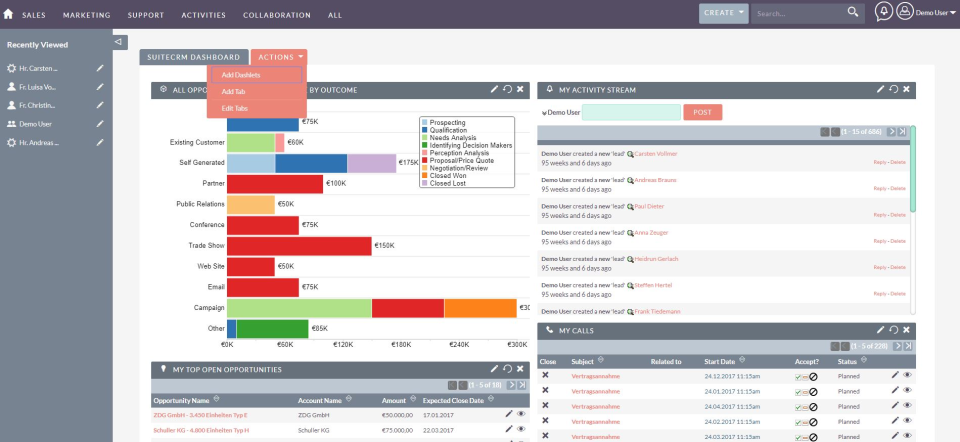
\includegraphics[scale=0.25]{sgeI/suiteCRM.jpg}
    \caption{Interfaz de SuiteCRM}
    \label{fig:my_label}
\end{figure}
\newpage
\section{CRM Propietario: SalesForce Sales Cloud}
\subsection{Información general}
SalesForce Sales Cloud es el CRM de SalesForce. El ecosistema SalesForce se encuentra en la versión Spring 22', \\ La mayor característica de este CRM es su personalización. Este CRM tiene varias versiones a contratar: 
\begin{itemize}
    \item Group
    \item Professional
    \item Enterprise
    \item Unlimited
    \item Performance
\end{itemize}
Además de tres niveles de atención por parte de la empresa: 
\begin{itemize}
    \item Standard Success Plan
    \item Premier Success Plan
    \item Premier+ Success Plan.
\end{itemize}
Estando todas ellas ordenadas de menor a mayor atención y precio.\\El CRM es vendido como un Software como servicio, es decir, pagas mensualmente y tienes la atención de la empresa. 
\subsection{Módulos y aplicaciones}
Este CRM tiene diversos módulos, entre ellos: 
\begin{itemize}
    \item  Marketing
    \item Ventas
    \item Atención al usuario
    \item Analíticas del negocio
\end{itemize}
En la atención al usuario se presta atención tanto a B2B (\textit{Business to business}, Negocio a negocio) como a B2C (\textit{Business to customer}, Negocio a cliente).\\ 
Con estos módulos uno puede, desde un mismo sitio, manejar los principales asuntos de la empresa. Además, dispone de una tienda de aplicaciones llamada 'AppExchange', por lo que puedes acceder a decenas de aplicaciones necesarias.
\newpage
\subsection{Hardware y software}
Una de las grandes ventajas de este CRM es que no necesita ni hadware ni software, al estar todo integrado en el navegador web.  

\subsection{Interfaz gráfica}
SalesForce Sales Cloud tiene una versión de navegador y otra de móvil. 
\begin{figure}[h]
    \centering
    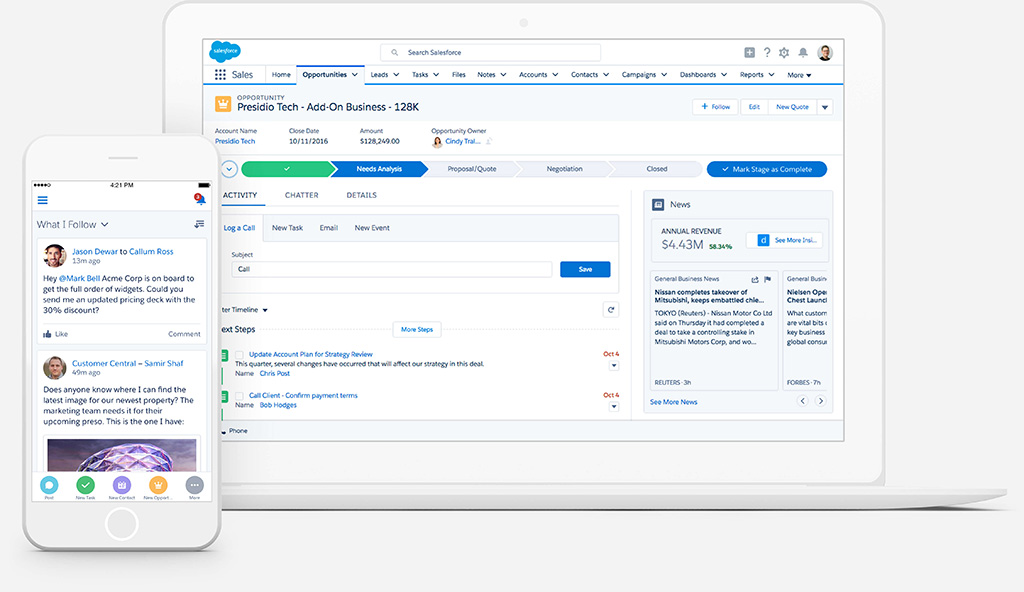
\includegraphics[scale=0.4]{sgeI/Salesforce.jpg}
    \caption{Interfaz de SalesForce, tanto de su versión de navegador como de su versión móvil}
    \label{fig:my_label}
\end{figure}
\addcontentsline{toc}{chapter}{Bibliografía}
\begin{thebibliography}{X}
\bibitem{Baz} \textsc{Módulos de Odoo}:
\textit{\url{https://www.bistasolutions.com/resources/blogs/odoo-modules-list/}}
\bibitem{Baz} \textsc{Odoo Hardware, IoT}:
\textit{\url{https://www.odoo.com/es_ES/app/point-of-sale-hardware}}
\bibitem{Baz} \textsc{Odoo Hardware, general}:
\textit{\url{https://www.odoo.com/es_ES/app/inventory-hardware}}
\bibitem{Baz} \textsc{Odoo, usuarios simultáneos}:
\textit{\url{https://www.odoo.com/es_ES/forum/ayuda-1/how-much-users-maximum-is-handle-in-odoo-101703}}
\bibitem{Baz} \textsc{SuiteCRM, store}:
\textit{\url{https://store.suitecrm.com/suitecrm-modules}}
\bibitem{Baz} \textsc{SuiteCRM, usuarios simultáneos}:
\textit{\url{https://store.suitecrm.com/addons/suitecrm-simultaneous-logins}}
\bibitem{Baz} \textsc{SuiteCRM, requerimientos}:
\textit{\url{https://community.suitecrm.com/t/minimum-server-droplet-requirements/58110/3}}
\bibitem{Baz} \textsc{SAP, Hardware}:
\textit{\url{https://help.sap.com/viewer/4b99f675d74f4990b75a8630869a0cd2/CURRENT_VERSION/en-US/526e0e40a177492198d44419db83c817.html}}
\bibitem{Baz} \textsc{SAP, información general}:
\textit{\url{https://www.udemy.com/course/sap-conceptos-e-iniciacion/}}
\bibitem{Baz} \textsc{SalesForce Sales Cloud, información general}:
\textit{\url{https://searchcustomerexperience.techtarget.com/definition/Salesforce-Sales-Cloud}}

\end{thebibliography}
\end{document}
